\documentclass[12pt]{article}

\usepackage{fullpage}
\usepackage{graphicx}
\usepackage{graphics}
\usepackage{mdwlist}


% christos: these look closer to NSF specs\dots
\setlength{\oddsidemargin}{0.0in}
\setlength{\evensidemargin}{0.0in}
\setlength{\textwidth}{6.5in}
\setlength{\headheight}{0.0in}
\setlength{\topmargin}{0.0in}
% \setlength{\textheight}{9.0in}
\setlength{\textheight}{9in}
\addtolength{\textheight}{-\topmargin}
\addtolength{\textheight}{-\headheight}
\addtolength{\textheight}{-\headsep}
\addtolength{\textheight}{-\footskip}



\begin{document}

\newcommand{\beq}{\begin{equation}}
\newcommand{\eeq}{\end{equation}}
\newcommand{\bit}{\begin{itemize*}}
\newcommand{\eit}{\end{itemize*}}
\newcommand{\goal}[1]{ {\noindent {$\Rightarrow$} \em {#1} } }
\newcommand{\hide}[1]{}
\newcommand{\comment}[1]{ {\footnotesize {#1} } }
\newtheorem{lemma}{Lemma}
\newtheorem{theorem}{Theorem}
\newtheorem{proof}{Proof}
\newtheorem{defn}{Definition}
\newtheorem{algo}{Algorithm}
\newtheorem{observation}{Observation}

\title{Multimedia Database Project Phase 1 Report}


\author{ {\em Jiajun Wang} \\
	    {\tt jiajunwa@andrew.cmu.edu}
	 \and
	 {\em San-Chuan Hung} \\
	     {\tt sanchuah@andrew.cmu.edu}
}

\maketitle
\section{Literature Survey}
    \label{sec:survey}
    Next we list the papers that each member read,
along with their summary and critique.

\subsection{Papers read by Jiajun Wang}
The first paper was the wavelet paper by Kang et al.
\cite{Daubechies92Ten}
\begin{itemize*}
\item {\em Main idea}: This paper proposes a graph mining package named PEGASUS, which performs multiple graph mining tasks based on Hadoop platform. The core innovation of PEGASUS improves graph mining performance by using MapReduce.
In order to achieve this, the paper firstly summarizes different mining operations and models these operations into a matrix-vector multiplication expression, which is called "Generalized Iterative Matrix-Vector multiplication" (GIM-V). GIM-V focuses on typical datasets consistent with node and edge data. It requires 3 processing steps: "combine2", "combineAll", "assign". On one side, these 3 steps are mapped to matrix-vector multiplication. On the other side, these 3 steps can be mapped to different MapReduce stages. According to the definition, we can find that GIM-V steps are strongly related with map-reduce processes. Particularly, "combine2" can be done using a map-reduce process and then the output is sent to another map-reduce process, which implement "combineAll"/"assign" functions. The basic version of this implementation is called "GIM-V Base".
Secondly, the paper discusses how to improve the basic version of GIM-V. Following methods are discussed: 1. Block Multiplication (Perform GIM-V on non-zero blocks, which forces co-locating and shorten sorting time). 2. Clustered Edges (Preprocessing for clustering edge files for better performance). 3. Diagonal Block Iteration (Preprocessing diagonal blocks to reduce iteration). 4. Node Renumbering (Make the minimum node located at the center of the graph to reduce iteration).
Thirdly, the paper analyzes and evaluates the performance of GIM-V with different improving methods. The experiments compared different scenarios from 2 aspects. The first one is scalability. We can see from the chart that the run time of GIM-V is decreased while the number of machines is increased. The second one is comparing between different GIM-V versions. We can see that basically, GIM-V BL-CL out performs other methods.
Finally, GIM-V is applied into real world tasks to check usability.
\item {\em Shortcomings}:
	For future research, I think besides finding more ways to improve the algorithm, this package can also be enhanced at the system layer. For handling very large graph data more efficiently, we can customize Hadoop system so as to optimize disk IO and cache.
\end{itemize*}

The second paper was by Kang et al.
\cite{Daubechies92Ten}
\begin{itemize*}
\item {\em Main idea}: This paper introduces GBASE, which supports both storing and querying for large-scale graph data. The main focuses of GBASE are faster query while using less storage space. Basically, GBASE reaches this goal by using parallel processing and distributed compressed storage based on MapReduce framework.
Firstly, in order to save graph data more efficiently, GBASE requires the data to be compressed. By assuming the data set has homogeneous block, the paper proposes block based compression algorithms?which ignore empty blocks and encode informative blocks. The interesting thing here is that although compressing and uncompressing data cost extra time, this method does not affect overall query response time. Because compressed data is much smaller than original one. Another fact that enhances query is the way GBASE stores data. After compression, the data is stored following "Grid placement". Which maximizes data localization and minimize the accessed files during query.
Secondly, the paper analyzes nature of supported graph queries. By leveraging MapReduce framework, GBASE implements efficient scalable graph queries.
Finally, GBASE is evaluated using large graph data. The results of the experiments show two things. Initially, compression plays very important role in both storage saving and query performance enhancement. We see the data storage consumption is reduced 43x. Next, MapReduce framework does provide scalability. Big data set is processed faster when increase machines.
\item {\em Shortcomings}:
	One problem of this paper may be the assumption of homogeneous block. For a random graph data, block compression may not work well. But on the other hand, this fact means GBASE can handle graph that has homogeneous blocks very effectively.
	Another point for future work in my opinion is using cache to accelerate compression/decompression process to further improve the query response time.
\end{itemize*}


The third paper was by Kang et al.
\cite{Daubechies92Ten}
\begin{itemize*}
\item {\em Main idea}:This paper introduces a new graph mining algorithm package named HADI, which is designed to estimate diameter and radius of large graphs. The key points of HADI are 1. approximation instead of calculate the exact value, 2. The algorithm is scalable and could be applied to MapReduce framework. These innovations optimize the algorithm performance. So HADI is able to handle massive data in reasonable time.
In the first part, the author defines effective radius and diameter for approximation. Basically, the algorithm will take 90\% as a threshold. And the result can still keep the important information about the graph. Then a scalable algorithm based on Flajolet-Martin algorithm is proposed. This algorithm requires O(n log n) space so it cannot be executed in a single machine for big data input.
Subsequently, the author introduces HADI algorithm. It is a disk-based algorithm so as to deal with large graph. Initially, a 2 stages algorithm HADI-naive is illustrated. Naive method divides previous algorithm in to a 2 phases MapReduce process. But it is not efficient enough. Then improved version of HADI algorithm is proposed. The basic idea is using an extra MapReduce phase to illuminate the copying unnecessary bitstrings. Moreover, 2 more optimizations are applied for handling block operations and compress the input size. As a result, HADI achieves O(d(m+n)/M log (m+n)/M) time complexity and O((m+n) log n) space complexity (n for nodes number, m for edges number and d for diameter).
Thirdly, the paper reports lot of experiment results to prove the stability and efficiency of HADI. We can see that using more nodes will shorten the running time of the algorithm. Although it is not linear related due to the overhead of the framework, the chart is persuasive to show the scalability. On the other hand, comparing between different optimized versions show that the final version works much better than the naive one.
Finally, the author applied HADI on real world data and found interesting result. It demonstrates the power of HADI and validates effective radius and diameter definition.
\item {\em Shortcomings}:
	For the future work, besides including more graph mining operations and supporting larger data size, I think the author can also try to leverage some in-memory distributed database for overcoming the shortage of disk-based.
\end{itemize*}


\subsection{Papers read by San-Chuan Hung }
The first paper was the wavelet paper by Alvarez-Hamelina et al.
\cite{Daubechies92Ten}
\begin{itemize*}
\item {\em Main idea}: The work proposed a large-scale graph visualization algorithm based on k-core. K-core means a sub-graph where the degrees of the nodes in the sub-graph are equal or higher than k. The visualization algorithm plots the points in the highest k-core to the center of the graph, and then plots the points in the second-highest k-core around previous highest k-core points, and so on.
\item {\em Shortcomings}:
		\begin{itemize*}
		\item
			The visualization algorithm may not be able to present the importance of "weak links," because the degree of the nodes in weak links may be not large enough to be shown in k-core algorithm. For example, for a bridge node whose degree is 2 but linking two large components, the node will not be focused because it?s coreness is low.
		\item
			The links are not weighted in the proposed algorithm. In some cases, the weights on links matter (for example, the intersect holding networks of companies); however, the proposed visualization algorithm dose not utilize link weights.
		\item
			In the proposed algorithm, it just random sampled the links to present.  As it was mentioned in the paper, edge reduction can be more sophisticated to emphasize the connections between groups or nodes. For example, it can just present important (high betweenness) edges.
		\end{itemize*}
\end{itemize*}

The second paper was by Kang et al.
\cite{Daubechies92Ten}
\begin{itemize*}
\item {\em Main idea}: The work proposed a framework for graph mining called HEIGEN to utilize Hadoop to do spectral analysis on large-scale data. Especially, HEIGEN accelerates the efficiency by choosing right part of operations to parallelize and reducing network traffic by dividing adjacency matrix into blocks. HEGIEN is useful for finding clusters and calculating triangles in large graphs.
\item {\em Shortcomings}:
		\begin{itemize*}
		\item
			Maybe HEIGEN can be shifted to memory-based map-reduce framework, like Spark, which is more efficient than Hadoop.
		\end{itemize*}
\end{itemize*}

The third paper was by Koutra et al.
\cite{Daubechies92Ten}
\begin{itemize*}
\item {\em Main idea}: The work compares different label propagation models, predicting the label of nodes in a graph by propagating known node labels through links, like Random Walk with Restarts, Semi-Supervised Learning and Belief Propagation(BP). It also proposed FABP model, implementing modified BP model in Hadoop framework, which is scalable, as accurate as BP model, and faster than BP model.
\item {\em Shortcomings}:
		\begin{itemize*}
		\item
			The experiments of FABP in this paper are mainly two-classes label classification (AI papers vs. NOT AI papers, Educational websites vs. Adult websites). I think future experiments can test FABP on multiple-classes label cases, like predicting websites is Adult/Educational/Financial.
		\end{itemize*}
\end{itemize*}

\section{K-cores Algorithm Implementation}
    \label{sec:proposed}
    
We implemented k-cores algorithm in gm\_main.py, in which the function name is "k\_core". Please see the implementation in the zip file of code.  

\section{Unit Test}
    \label{sec:experiments}
    We implemented our method
and compared it with the older ones.
The results are very promising.

\section{Connected Component}
\begin{itemize*}
\item {Case 1 All separate graph.}
Input:
1, 2
3, 4
5, 6
7, 8

Output:
8	7
4	3
1	1
5	5
3	3
6	5
2	1
7	7
\end{itemize*}


\begin{figure}[htbf]
\begin{center}
\begin{tabular}{cc}
     % uncomment the next lines, and give the right ps files
     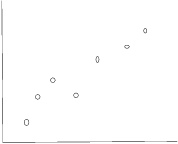
\includegraphics[width=0.3\textwidth]{FIG/data.png} &
     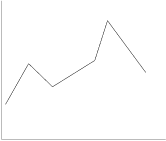
\includegraphics[width=0.3\textwidth]{FIG/plot.png} \\
     %\psfig{figure=FIG/plot.ps,width=2in} \\
     % \psfig{figure=FIG/data.ps,width=2in} &
     % \psfig{figure=FIG/plot.ps,width=2in} \\
    (a) & (b) 
\end{tabular}
\caption{A fictitious dataset (a) and its performance plot (b)}
\label{fig:results}
\end{center}
\end{figure}



\section{graphMiner Result}
    \label{sec:conclusions}
    The proposed method {\em someMETHOD}
has the following advantages:
\bit
\item it gives better classification accuracy than all 10 competitors we tried
\item its accuracy is very close to the very best competitor
      in the {\em UCR Insect Classification Contest}.
\item it is scalable
\eit


\bibliography{BIB/sanchuah}
\bibliographystyle{plain}

\newpage
\pagenumbering{roman}
\tableofcontents


\end{document}
